\documentclass[12pt]{article}
\usepackage{graphicx}

\newcommand{\PF}[1]{\marginpar{\tiny PF: #1}}

\begin{document}

\section{The DE10-nano board}

\subsection{Intel Cyclone V chip}
The DE10-nano development board is equipped with an FPGA from intel: Cyclone V. This chip is interesting because it not only contains an FPGA but also an ARM processor, it is a FPGA+SoC chip. The advantage of this style of architecture is to have on one side an OS such as linux that runs on a real processor and on the other side the possibility to configure a kind of peripheral on the FPGA side. Moreover, the circuits implemented on the FPGA side can be configured from the ARM processor side, which makes the FPGA part editable in real time. A very interesting example of use is hardware acceleration. One might want to create an audio system on the processor and need different calculation functions: Fourier transform, AC/DC converter, ... All these could simply be implemented by the ARM on the FPGA side whenever needed and use it afterwards if the FPGA space is critical. In the case space is not critical, all the operations can simply be permanently implemented on the FPGA. By doing this, it is often possible to reduce the number of atomic operations required for the complex operation implemented - the operation is now done in hardware and no longer in software.

\subsection{Peripherals}

\begin{figure}
  \center
  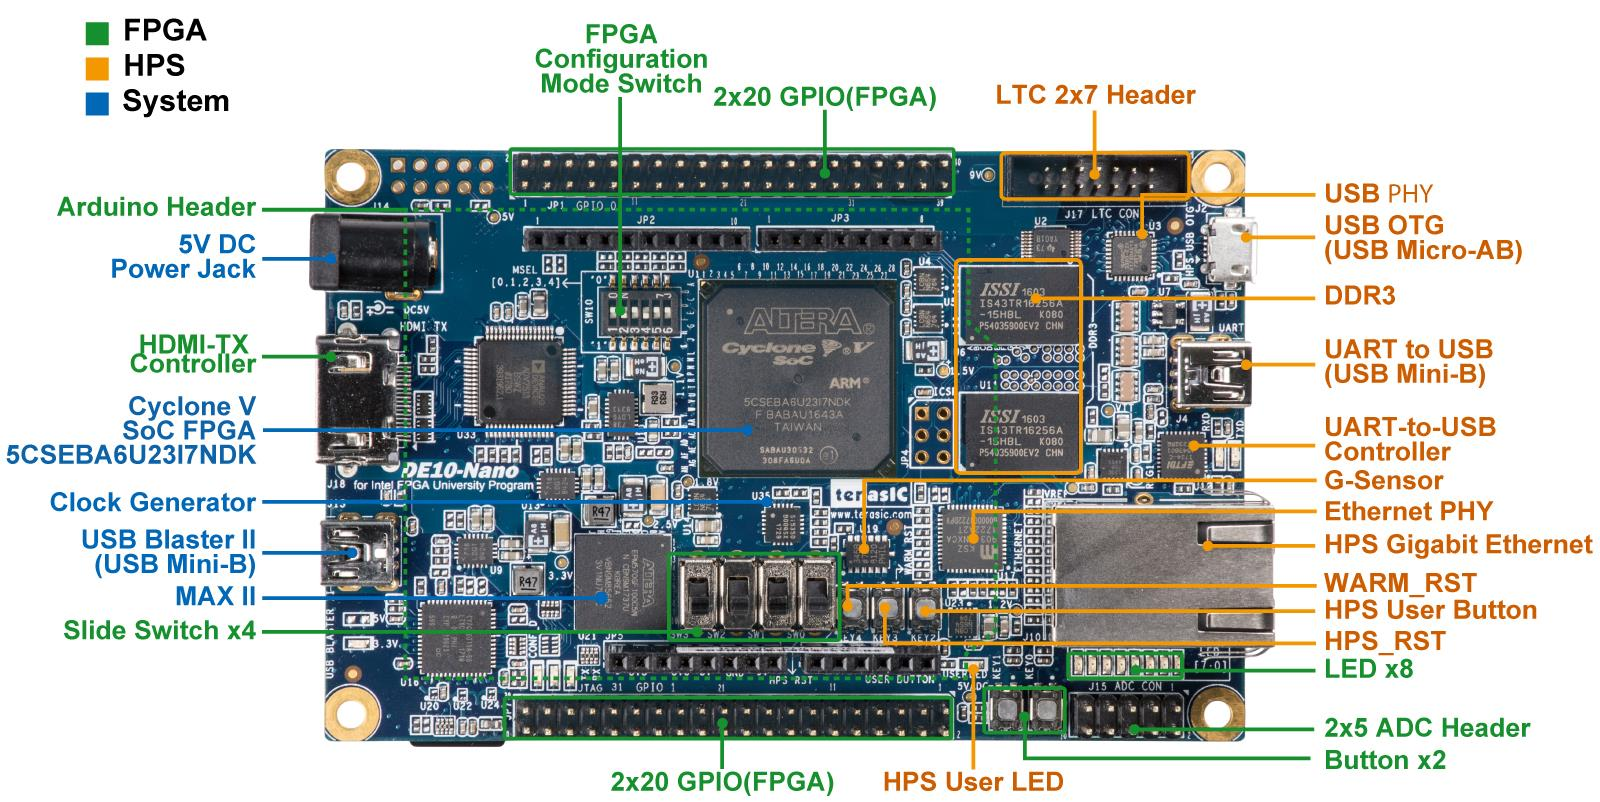
\includegraphics[width=15cm]{"res/chapter1/layout_components.png"}
  \caption{Layout and peripherals of the DE10-nano board}
  \label{fig:de10nano_peripherals}
\end{figure}

On the card, numerous peripherals are made available to the user. Some of them will be very interesting for this work: the DDR3 RAM memory, the SD card reader, the USB controller, as well as the HDMI output. Others allow to make tests, to check the operation without necessarily going through simulation. In this category, there are for example the General Purpose Input / Output pins (GPIOs), LEDs, buttons and sliders. And finally, there are other interesting peripherals that will not necessarily be used in this work such as the Inertial Measurement Unit (IMU) which contains gyroscopes, accelerometers and magnetometers and the ethernet controller.

\vspace{12pt}
All these devices are shown in the Figure \ref{fig:de10nano_peripherals}. It should be noted that the devices are always linked to one of the two parts of Cyclone-V. This means that the other part cannot access them directly. In order to access one of the peripherals on the other side, it will be necessary to use one of the bridges between the ARM part and the FPGA
part.

\subsection{Communication between ARM and FPGA sides}

TO BE COMPLETED AS SOON AS I AM ABLE TO ACCESS DDR3 MEMORY

\section{First implementation on the FPGA side}

As a first step, it was decided to verify that the use and implementation of circuits on the FPGA side was done in a traditional way. The first step was to create the top-level module and match its inputs and outputs to physical pins on the chip. These two steps were quickly completed using the system builder executable tool included in the development board CD-ROM provided by Terasic\footnote{Terasic is the manufacturer of the DE10-nano development board.}. A simple execution of this builder allows the generation of the project containing the mapping of the inputs and outputs as well as the top level module. Once this is done, it is possible to describe other modules and create an architecture to verify the functioning of the development chain of this FPGA.\PF{Please rephrase}

\subsection{8 bits counter with LEDs}

To check the development chain of this FPGA, an 8-bit counter has been implemented. This can be described very simply in verilog. As input this module takes the FPGA clock which oscillates at 50MHz and outputs the number contained in the 8-bit counter. The 8 bits are then mapped to the 8 LEDs on the board to make the number visible. However, with this update frequency, it is impossible to distinguish different numbers at the LEDs. The counter update frequency must therefore be reduced. An input is then added to the counter, the clock enable that will warn it when it needs to increment its value. To generate the clock enable, another module is implemented: the clock manager. This module is a counter that runs directly on the 50MHz except that it never returns its number. It will only count until it reaches a certain number that allows tuning the output frequency. In fact, as soon as the number is reached, the counter is reset to 0 and the clock enable goes to 1 for one clock tick. If the maximum number of the counter is set to $50 \times 10^6$, the clock enable will be generated once a second and the counter linked to the LEDs will be updated once a second as well. This makes reading at the LED level possible. The commented Quartus\footnote{Quartus Prime Lite 20.1 to be exact.} project of this subsection is available in \textsc{quartus/simple\_counter}.

\section{First implementation using both sides of the chip}

Now that a counter has been created, the idea will be to access the DDR3 RAM on the ARM side from the FPGA side. To do this, the bridges and the avalon bus must be handled. The goal is to put a number at startup in the RAM (this is done on the ARM side), get it from the FPGA part, load it into the counter and start counting from there. Finally, the count has to be updated in RAM by the FPGA. Doing this ensures that the communication between the two parts of the chip, in both directions, works.

\vspace{12pt}
TO BE COMPLETED AS SOON AS I AM ABLE TO ACCESS DDR3 MEMORY

\end{document}
